\question{Приложения определенного интеграла: вычисление площадей в декартовых координатах.}

\begin{figure}[H]
  \centering
  
  \begin{subfigure}[b]{0.3\textwidth}
  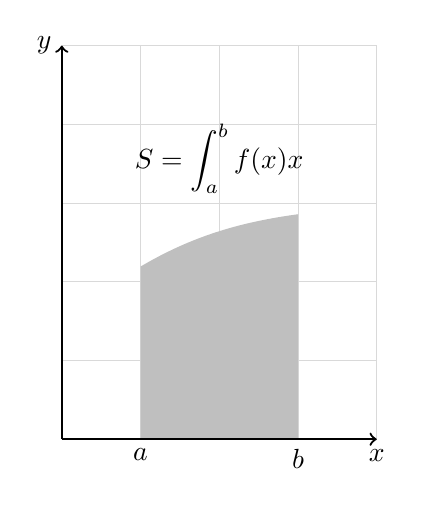
\begin{tikzpicture}
  
    \draw[very thin, gray!30, step = 1cm] (0, 0) grid (4, 5);
    \fill[lightgray, domain = 1 : 3, variable = \x]
      (1, 0)
      -- plot ({\x}, {3 / (1 + e^(-\x))})
      -- (3, 0)
      -- cycle;
  
    \draw[thick] [->] (0, 0) -- (4, 0) node[right, below] {\(x\)};
    \draw[thick] [->] (0, 0) -- (0, 5) node[above, left] {\(y\)};
    \draw node[above] at (2, 3) {\(\displaystyle
      S = \int_{a}^{b} f(x) \dd x
    \)};
    \draw node[below] at (1, 0) {\(a\)};
    \draw node[below] at (3, 0) {\(b\)};
  
  \end{tikzpicture}
  \caption{\(f(x) \ge 0\)}\label{fig:int-square-1}
  \end{subfigure}
  \qquad
  \begin{subfigure}[b]{0.3\textwidth}
    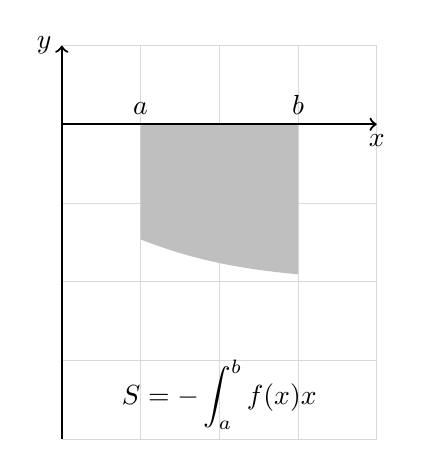
\begin{tikzpicture}
    
      \draw[very thin, gray!30, step = 1cm] (0, -4) grid (4, 1);
      \fill[lightgray, domain = 1 : 3, variable = \x]
        (1, 0)
        -- plot ({\x}, {-2 / (1 + e^(-\x))})
        -- (3, 0)
        -- cycle;
    
      \draw[thick] [->] (0, 0) -- (4, 0) node[right, below] {\(x\)};
      \draw[thick] [->] (0, -4) -- (0, 1) node[above, left] {\(y\)};
      \draw node[above] at (2, -4) {\(\displaystyle
        S = -\int_{a}^{b} f(x) \dd x
      \)};
      \draw node[above] at (1, 0) {\(a\)};
      \draw node[above] at (3, 0) {\(b\)};
    
    \end{tikzpicture}
    \caption{\(f(x) \le 0\)}\label{fig:int-square-2}
  \end{subfigure}
  \qquad
  \begin{subfigure}[b]{0.3\textwidth}
    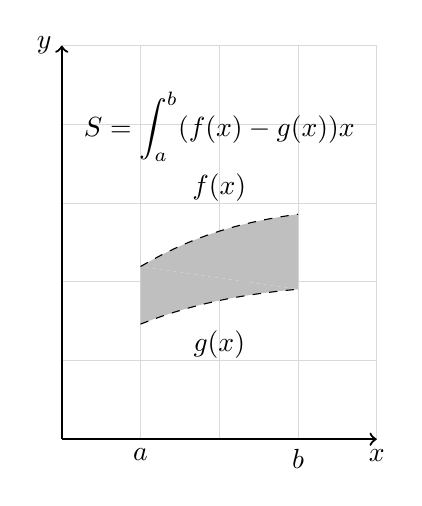
\begin{tikzpicture}
    
      \draw[very thin, gray!30, step = 1cm] (0, 0) grid (4, 5);
      \fill[lightgray, domain = 1 : 3, variable = \x]
        (1, 2.193)
        -- plot ({\x}, {3 / (1 + e^(-\x))})
        -- (3, 1.905);

      \fill[lightgray, domain = 1 : 3, variable = \x]
        (1, 1.462)
        -- plot ({\x}, {2 / (1 + e^(-\x))})
        -- (1, 2.193);

      \draw[dashed, domain = 1 : 3, variable = \x]
        plot ({\x}, {3 / (1 + e^(-\x))})
        node at (2, 3.2) {\(f(x)\)};
      \draw[dashed, domain = 1 : 3, variable = \x]
        plot ({\x}, {2 / (1 + e^(-\x))})
        node at (2, 1.2) {\(g(x)\)};
    
      \draw[thick] [->] (0, 0) -- (4, 0) node[right, below] {\(x\)};
      \draw[thick] [->] (0, 0) -- (0, 5) node[above, left] {\(y\)};
      \draw node[above] at (2, 3.4) {\(\displaystyle
        S = \int_{a}^{b} (f(x) - g(x)) \dd x
      \)};
      \draw node[below] at (1, 0) {\(a\)};
      \draw node[below] at (3, 0) {\(b\)};
    
    \end{tikzpicture}
    \caption{\(f(x) \ge g(x)\)}\label{fig:int-square-3}
  \end{subfigure}
\end{figure}

\begin{remark}
  Для случая \hyperref[fig:int-square-3]{(c)} расположение функций
  \(f(x)\), \(g(x)\) относительно нуля не важно. Важно лишь, чтобы
  \(\forall x \in [a; b] \colon f(x) \ge g(x)\).
\end{remark}